\chapter{Introduction}\label{sec:introduction}

According to the latest Cisco's VNI \cite{video-traffic-forecast}, video will
account for 82\% of all IP traffic in Europe by 2021; in addition, the overall IP
traffic per person will triplicate from 13\emph{GB} to 35\emph{GB}. These
forecasts clearly picture the growth of the streaming industry, posing, at the
same time an important question on the present and future states of the final
user's privacy.

As shown by Reed et Al. \cite{netflix-real-time} anonimity of user's viewing
activity is at risk. Not for the use that Netflix or other streaming services
do of user's session data, but because of the risk of a man-in-the-middle
attack \emph{MITM} carried by an \textit{evil} party that has control over the
flow of packets over a network.

In particular, they have shown how the adoption of HTTPS to protect video
streams from Netflix \emph{CDN}s to user's end devices, does not hold against
passive traffic analysis.

\section{Motivation}\label{motivation}

The goal of this project is to replicate part of the work conducted by Reed et
Al. and to investigate the possibility of identifying a Netflix stream solely
based on the observed average bandwidth. This, follows from the intuition that
\emph{per-title encoding} embeds the nature and the complexity of video frames
in a unique way, that may reveal the identity of the content being streamed.

\subsection{Per-Title Encoding}\label{sec:per-title-encoding}

In December 2015 Netflix announced \cite{per-title-encoding} that it was
introducing a new method to analyze the complexity of each title and find the
best encoding recipe based on it. Their goal with the adoption of
per-title encoding was to provide users with better quality streams at a lower
bandwidth. 

Before then, each title was encoded with a \emph{Fixed Bitrate Ladder}; their
pipeline returned a list of \{\emph{Bitrate, Resolution}\} pairs that
represented the sufficient bitrate to encode the stream at a certain
resolution (\Cref{tab:fixed-ladder}), with no visible artificats.

\begin{table}[htb]
  \centering
  \begin{tabular}{|c|c|}
    \hline
    \textbf{Bitrate (kbps)} & \textbf{Resolution} \\
    \hline
    235                     &    $320\times240$ \\
    \hline
    375                     &    $384\times288$ \\
    \hline
    560                     &    $512\times384$ \\
    \hline
    750                     &    $512\times384$ \\
    \hline
    1050                    &    $640\times480$ \\
    \hline
    1750                    &    $720\times480$ \\
    \hline
    2350                    &   $1280\times720$ \\
    \hline
    3000                    &   $1280\times720$ \\
    \hline
    4300                    &   $1920\times1080$ \\
    \hline
    5800                    &   $1920\times1080$ \\
    \hline
  \end{tabular}
  \caption{Netflix original's Fixed Bitrate Ladder.}
  %\end{center}
  \label{tab:fixed-ladder}
\end{table}

This "one-size-fits-all" ladder, as reported, achieved good results in the
encoded video's perceived quality (\textbf{PSNR} \cite{psnr}) given the bitrate
constraint, but, would not perform optimally under certain conditions. For
instance, high detailed scenes with sudden changes of light, or rapid
transitions of camera shots, would require more than 5800\emph{kbps}; in
contrast, more static frames, as in animated cartoons, may be encoded at higher
resolutions mantaining the same bitrate level.

In summary they noticed how in certain cases, the produced encoding would
either present some small artifacts (\emph{e.g.} complex scenes), or waste
bandwidth, (\emph{e.g.} static, plain scenes). For this reason, they came up
with per-title encoding.

\begin{table}[htb]
  %\begin{center}
  \centering
  \begin{tabular}{|c|c|c|}
    \hline
    \textbf{Resolutions} & \textbf{Fixed Bitrate Ladder (kpbs)} & \textbf{Per-Title Bitrate Ladder (kbps)} \\
    \hline
    $320\times240$       & 235                                  & 150 \\
    \hline
    $384\times288$       & 375                                  & 200 \\
    \hline
    $512\times384$       & 560                                  & 290 \\
    \hline
    $512\times384$       & 750                                  & \\
    \hline
    $640\times480$       & 1050                                 & \\
    \hline
    $720\times480$       & 1750                                 & 440\\
    \hline
    $720\times480$       &                                      & 590\\
    \hline
    $1280\times720$      & 2350                                 & 830\\
    \hline
    $1920\times1080$     & 3000                                 & 1150\\
    \hline
    $1920\times1080$     & 4300                                 & 1470\\
    \hline
    $1920\times1080$     & 5800                                 & 2150\\
    \hline
    $1920\times1080$     &                                      & 3840\\
    \hline
  \end{tabular}
  \caption{
    Comparison between the two different approaches for the same title: note
    how different titles may have different numbers of quality levels. For each
    movie, the minimum number of quality levels gets computed to produce a
    just-noticeable-difference (JND), when switching bitrates during playback.
  }
  \label{tab:old-vs-new-ladder}
\end{table}

In order to find the best fitting bitrate ladder for a particular title, there
are several criterias that they took into account, the principal ones being:

\begin{itemize}
    \item How many quality levels should be encoded to obtain a
          \emph{JND} between each of them.
    \item Best \{\emph{Resolution, Bitrate}\} pair for each quality level
    \item Highest bitrate required to achieve the best perceivable quality
\end{itemize}

As aforementioned, each title's perceived video quality, gets computed as a
measure of \emph{Peak signal-to-noise ratio}. The comparison is performed
between the produced encode, upsampled to 1080\emph{p}, and the original title
in 1080\emph{p}, and the best \{\emph{Bitrate, Resolution}\} pair is assigned
to that specific quality level, as depicted in \Cref{tab:old-vs-new-ladder}.

In \Cref{fig:new-vs-old-ladder}, we can see the impact of per-title encoding on
the original bitrate ladder: in order to achieve the same perceivable quality
level (point \textbf{B} and \textbf{C}), it requires a lower bitrate to be
encoded to (point \textbf{A}).  Moreover, with around the same bitrate, one can
see how per-title encoding can achieve a higher resolution compared the fixed
case (point \textbf{A} and \textbf{D} respectively). It follows obviously that,
holding to a high-quality stream while maintainig or lowering the used
bandwidth is key: the end user will get same or better quality then before, at
a lower bandwidth.

\begin{figure}[!htb]
  \centering
  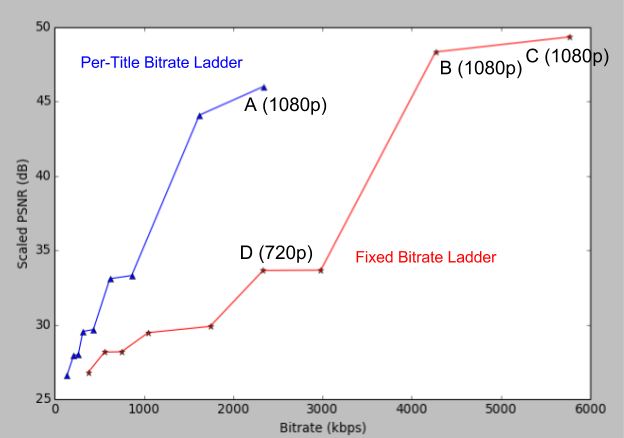
\includegraphics[width=0.9\columnwidth]{img/pertitlevsfixed.png}
  \caption{Difference between per-title vs. fixed bitrate ladders.}
  \label{fig:new-vs-old-ladder}
\end{figure}

\subsection{User's Privacy}\label{sec:privacy}

As of 2018, data began the most valuable commodity on the planet
\cite{data-value}, and with its value rising, society starts to question how to
legislate to protect both industry's and user's rights.

In 2016, Netflix announced the introduction of HTTPS to protect the content
being streamed to users. With the addition of TLS on top of HTTP, Netflix aim,
was to avoid the risk of eavesdropping on unsecure connections, protecting
themselves and users from third-party applications and governments potentially
collecting viewer's data and streaming habits.

Avoiding deep packet inspection from potential eavesdropper certainly adds
another layer of security, but given the narrow relationship between Netflix
and ISPs, one might conclude that the chance that IP packets do not get
inspected by ISPs (especially in the United States, after the reclassification
of ISPs as Title I \emph{Information Services} \cite{net-neutrality}), is still
a matter of mere trust given to the platform-provider relationship.

Cases of user's data breaches as the Kanopy one \cite{kanopy}, are a testimony
of how easy would be for an attacker to extract information to the point at
which users could become identifiable by the solely information the platform
was collecting in their internal log files. The content of which, include
between others: timestamps, geo-location data, client-device informations and
IP addresses. 

The ability to cluster people based on just their video-streaming habits, poses
a potential threat for how the data could be processed and used by parties with
access to it. One could imagine how government agencies could easily get in
possession of sensitive information about the nature of the content a
particular user is interested about, or how ISPs could profit from selling data
profiles to advertisement companies that in turn would exploit their
information to improve per-user recommendation algorithms.

Considering this trend, it is for us crucial to investigate how parties that
can have access to transport-layer information, (more details in
\Cref{sec:approach}), could exploit per-title encoding to identify video
traffic. 

\section{Related Work}\label{related}

\todo{add more}

As previously mentioned, our work is mainly insipired by Reed et Al.'s
\cite{netflix-real-time} research paper, in which they presented a novel method
to de-anonymize encrypted netflix stream in real-time with limited hardware
requirements. Their system was able to identify a video using uniquely TCP/IP
headers, by making use of \texttt{adudump}, a command-line program built on top
of \emph{libpcap} \cite{libpcap}, a powerful C library for network traffic
capture. They acquired for each video, metadata information with a tampering
tool, and then matched adudump traces against with. The evaluation of their
method revelaed that they could identify majority of videos by recording only
20 minutes of traffic each.

An earlier proof on how bandwidth analysis could reveal the content of
ecnrypted traffic, was given by Saponas et Al. \cite{Saponas2007devices}, in
their "SlingBox-Pro" case study, that exposed how, by recording network traffic
and producing and combining different trace levels, they were able to identify
98\% of 40 minutes video traces.

Similar work has been conducted also by Moser \cite{moser}, who analyzed how
bitrate ladders could uniquely embed the identity of Netflix titles. In his
work he further studies the impact of the aggregation of each video's segment
bandwidth on the overall accuracy of his system. 

\section{Main Objective}\label{sec:objective}

The main goal of this project is to build a system that can manipulate network
bandwidth and observe video traffic from Netflix, to verify the intuition that
each title could be identified by its own bitrate ladder. 

Furthermore we investigate and discuss possible countermeasures that streaming
providers could adopt to preserve users privacy. A detailed explanation of our
approach is presented in \Cref{sec:approach}

\section{Structure of this Report}\label{sec:structure}
  
In this section, we outline the contents and the structure of this report.

\Cref{sec:introduction} introduced our motivation behind the project, presented featured work
that influenced and inspire our approach, and listed the goals we would like to
ultimately achieve.

\Cref{sec:attack_isp} presents the attack scenario from a perspective of a
malicious user that has compromised a node on the path between the client and
the server), the infrastructure needed to acquire the data, the nature of the
information that could be infered, and the consequences that might arise.

\Cref{sec:approach} shows our version of the attack, in a different context, but up to
some extent, with similar conditions to the one depicted in Chapter 2. It also
higlights the similiarities and differences from the featured approaches we
followed.

\Cref{sec:results} we evaluate our system, we present results, and discuss the
relevance of such a method.

\Cref{sec:conclusion} tries to summarize and draw conclusions based on the claims made at
the beginning of this report.
%TODO Chapter 2 - End to End Attack Scenario 
               %- Describe the attack scenario from the perspective of an ISP
               %- Describe the infrastructure
               %- Describe what kind of information the attacker is able to retrieve
               %- Outline the consequences of such an attack
%TODO Chapter 3 - Approach
               %- Present our version of the attack scenario
               %- Describe the infrastructure
               %- Present the data we have collected
               %- Highlight the differences from our approach to Reed's et Al.
               %- Explain how we can uniquely identify a movie / Explain how we
                  %make use of the features we collect
%TODO Chapter 4 - Evaluation of the system
               %- Explain Plots & result data
%TODO Chapter 5 - Conclusion
               %- Future Work
               %- Acknowlegments
